\clearpage
\section{标签提取与双向匹配设计}
\label{sec:design-matching}
介绍里有两类信息，一类描述用户本人，一类描述希望遇到的人。用户提交有效介绍并同意展示后，系统先保存原文，再从固定词表中提取本人标签和期望标签。

\begin{figure}[H]
\centering
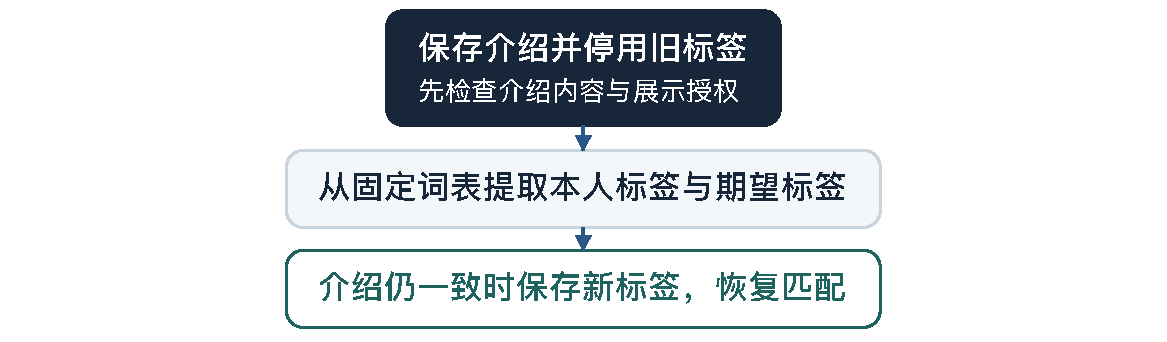
\includegraphics[width=\linewidth]{assets/design/tag-matching.pdf}
\caption{从介绍提交到匹配资料就绪的更新流程}\label{fig:design-tags}
\end{figure}

修改介绍后，旧标签先退出匹配。等提取结果对应的介绍与当前介绍一致，账号才重新参与匹配。记用户 $a$ 的本人标签为 $S_a$、期望标签为 $D_a$，候选 $b$ 的标签同样记。下面分别计算两个人的期望满足率。
\begin{equation}
 r_{a\to b}=\frac{|D_a\cap S_b|}{|D_a|},\qquad
 r_{b\to a}=\frac{|D_b\cap S_a|}{|D_b|}.
\end{equation}
\begin{equation}
M(a,b)=\begin{cases}
0,&r_{a\to b}r_{b\to a}=0,\\
\operatorname{round}[50(r_{a\to b}+r_{b\to a})],&\text{其余}.
\end{cases}\label{eq:design-match}
\end{equation}
标签就绪、期望标签非空后才能算分。只要有一方的期望与对方标签完全不重合，分数就是0。其余情况取两个满足率的平均值，换算成整数分。

\begin{table}[H]
\centering\small
\caption{双向满足率对候选资格的影响算例}\label{tab:design-match-examples}
\begin{tabularx}{\linewidth}{@{}p{27mm}p{27mm}p{20mm}X@{}}
\toprule 本人期望满足率 & 对方期望满足率 & 匹配分 & 候选判断 \\ \midrule
$2/3$ & $1/2$ & 58 & 低于60分，过滤 \\
$3/4$ & $1/2$ & 63 & 通过分数条件，仍需资格过滤 \\
$1$ & $0$ & 0 & 单向满足，不进入候选池 \\
\bottomrule
\end{tabularx}
\end{table}
匹配分达到60后，还需按收藏、冷却和联系状态筛选。卡片上展示的是本人期望标签与对方本人标签的交集。用户可以先看具体有哪些标签重合，再决定要不要发纸条。

